% THIS DOCUMENT IS TAILORED TO REQUIREMENTS FOR SCIENTIFIC COMPUTING.  IT
% SHOULDN'T BE USED FOR NON-SCIENTIFIC COMPUTING PROJECTS
\documentclass[12pt]{article}

\usepackage{amsmath, mathtools}
\usepackage{amsfonts}
\usepackage{amssymb}
\usepackage{graphicx}
\usepackage{colortbl}
\usepackage{xr}
\usepackage{hyperref}
\usepackage{longtable}
\usepackage{xfrac}
\usepackage{tabularx}
\usepackage{float}
\usepackage{siunitx}
\usepackage{booktabs}
\usepackage{caption}
\usepackage{pdflscape}
\usepackage{afterpage}
\usepackage{cite}

%\usepackage[round]{natbib}

%\usepackage{refcheck}

\hypersetup{ bookmarks=true,         % show bookmarks bar?
      colorlinks=true,       % false: boxed links; true: colored links
    linkcolor=red,          % color of internal links (change box color with
                            % linkbordercolor)
    citecolor=green,        % color of links to bibliography
    filecolor=magenta,      % color of file links
    urlcolor=cyan           % color of external links
}

%% Comments

\usepackage{color}

\newif\ifcomments\commentstrue %displays comments
%\newif\ifcomments\commentsfalse %so that comments do not display

\ifcomments
\newcommand{\authornote}[3]{\textcolor{#1}{[#3 ---#2]}}
\newcommand{\todo}[1]{\textcolor{red}{[TODO: #1]}}
\else
\newcommand{\authornote}[3]{}
\newcommand{\todo}[1]{}
\fi

\newcommand{\wss}[1]{\authornote{blue}{SS}{#1}} 
\newcommand{\plt}[1]{\authornote{magenta}{TPLT}{#1}} %For explanation of the template
\newcommand{\an}[1]{\authornote{cyan}{Author}{#1}}

%% Common Parts

\newcommand{\progname}{ProgName} % PUT YOUR PROGRAM NAME HERE
\newcommand{\authname}{Team \#, Team Name
\\ Student 1 name
\\ Student 2 name
\\ Student 3 name
\\ Student 4 name} % AUTHOR NAMES                  

\usepackage{hyperref}
    \hypersetup{colorlinks=true, linkcolor=blue, citecolor=blue, filecolor=blue,
                urlcolor=blue, unicode=false}
    \urlstyle{same}
                                


% For easy change of table widths
\newcommand{\colZwidth}{1.0\textwidth}
\newcommand{\colAwidth}{0.13\textwidth}
\newcommand{\colBwidth}{0.82\textwidth}
\newcommand{\colCwidth}{0.1\textwidth}
\newcommand{\colDwidth}{0.05\textwidth}
\newcommand{\colEwidth}{0.8\textwidth}
\newcommand{\colFwidth}{0.17\textwidth}
\newcommand{\colGwidth}{0.5\textwidth}
\newcommand{\colHwidth}{0.28\textwidth}

% Used so that cross-references have a meaningful prefix
\newcounter{defnum} %Definition Number
\newcommand{\dthedefnum}{GD\thedefnum}
\newcommand{\dref}[1]{GD\ref{#1}} \newcounter{datadefnum} %Datadefinition Number
\newcommand{\ddthedatadefnum}{DD\thedatadefnum}
\newcommand{\ddref}[1]{DD\ref{#1}} \newcounter{theorynum} %Theory Number
\newcommand{\tthetheorynum}{TM\thetheorynum}
\newcommand{\tref}[1]{TM\ref{#1}} \newcounter{tablenum} %Table Number
\newcommand{\tbthetablenum}{TB\thetablenum}
\newcommand{\tbref}[1]{TB\ref{#1}} \newcounter{assumpnum} %Assumption Number
\newcommand{\atheassumpnum}{A\theassumpnum}
\newcommand{\aref}[1]{A\ref{#1}} \newcounter{goalnum} %Goal Number
\newcommand{\gthegoalnum}{GS\thegoalnum}
\newcommand{\gsref}[1]{GS\ref{#1}} \newcounter{instnum} %Instance Number
\newcommand{\itheinstnum}{IM\theinstnum}
\newcommand{\iref}[1]{IM\ref{#1}} \newcounter{reqnum} %Requirement Number
\newcommand{\rthereqnum}{R\thereqnum}
\newcommand{\rref}[1]{R\ref{#1}} \newcounter{nfrnum} %NFR Number
\newcommand{\rthenfrnum}{NFR\thenfrnum}
\newcommand{\nfrref}[1]{NFR\ref{#1}} \newcounter{lcnum} %Likely change number
\newcommand{\lthelcnum}{LC\thelcnum}
\newcommand{\lcref}[1]{LC\ref{#1}}

\usepackage{fullpage}

\newcommand{\deftheory}[9][Not Applicable]
{ \noindent \rule{\textwidth}{0.5mm}

\paragraph{RefName: } \textbf{#2} \phantomsection 

\paragraph{Label:} #3
\label{#3}

\noindent \rule{\textwidth}{0.5mm}

\paragraph{Equation:}

#4

\paragraph{Description:}

#5

\paragraph{Notes:}

#6

\paragraph{Source:}

#7

\paragraph{Ref.\ By:}

#8

\paragraph{Preconditions for \hyperref[#2]{#2}:}
\label{#2_precond}

#9

\paragraph{Derivation for \hyperref[#2]{#2}:}
\label{#2_deriv}

#1

\noindent \rule{\textwidth}{0.5mm}

\newpage

}

\begin{document}

\title{Software Requirements Specification for \progname: subtitle describing software} 
\author{\authname}
\date{\today}
	
\maketitle

~\newpage

\pagenumbering{roman}

\tableofcontents

~\newpage

\section*{Revision History}

\begin{tabularx}{\textwidth}{p{3cm}p{2cm}X} \toprule {\bf Date} & {\bf Version}
& {\bf Notes}\\
\midrule
January 16, 2025 & 1.0 & Creation\\
\bottomrule
\end{tabularx}

~\\

~\newpage

\section{Reference Material}

This section records information for easy reference.

\subsection{Table of Units}

Throughout this document SI (Syst\`{e}me International d'Unit\'{e}s) is employed
as the unit system.  In addition to the basic units, several derived units are
used as described below.  For each unit, the symbol is given followed by a
description of the unit and the SI name.  ~\newline

\renewcommand{\arraystretch}{1.2}
%\begin{table}[ht]
  \noindent \begin{tabular}{l l l} 
    \toprule		
    \textbf{symbol} & \textbf{unit} & \textbf{SI}\\
    \midrule 
    \si{\second} & time & second\\
    \si{\volt} & voltage & volt\\
    \si{\hertz} & frequency & hertz (\si{\hertz} = \si{\per\second})\\
    \bottomrule
  \end{tabular}
  %	\caption{Provide a caption}
%\end{table}
~\newline

\noindent Exceptionally, some units officially accepted for use with the SI are
used as described below.  ~\newline

\renewcommand{\arraystretch}{1.2}
%\begin{table}[ht]
  \noindent \begin{tabular}{l l} 
    \toprule		
    \textbf{symbol} & \textbf{unit}\\
    \midrule 
    \si{\decibel} & logarithmic ratio quantity\\
    \bottomrule
  \end{tabular}
  %	\caption{Provide a caption}
%\end{table}

\subsection{Table of Symbols}

The table that follows summarizes the symbols used in this document along with
their units.  The choice of symbols was made to be consistent with the existing
documentation for the R-wave detector.  The symbols are listed in alphabetical
order.

\renewcommand{\arraystretch}{1.2}
%\noindent \begin{tabularx}{1.0\textwidth}{l l X}
\noindent \begin{longtable*}{l l p{12cm}} \toprule \textbf{symbol} &
\textbf{unit} & \textbf{description}\\
\midrule 
$a$ & N/A & a sequence of digital filter weighting coefficients \\
$A$ & \si{\mV} & a sequence of index of the annotated R wave \\
$b$ & N/A & a sequence of digital filter feedback coefficients \\
$f_c$ & \si{\hertz} & cutoff frequency of the filter \\
$f_s$ & \si{\hertz} & sampling frequency of the ECG signal \\
$H$ & N/A & transfer function of digital filter \\
$R$ & N/A & a sequence of index of the calculated R wave \\
$u$ & \si{\mV} & a sequence of discrete-time ECG signal \\
$z$ & N/A & complex frequency variable in the Z-domain, $z=e^{j2\pi f}$ \\
\bottomrule
\end{longtable*}

\subsection{Abbreviations and Acronyms}

\renewcommand{\arraystretch}{1.2}
\begin{tabular}{l l} 
  \toprule		
  \textbf{symbol} & \textbf{description}\\
  \midrule 
  A & Assumption\\
  DD & Data Definition\\
  GD & General Definition\\
  GS & Goal Statement\\
  IM & Instance Model\\
  LC & Likely Change\\
  PS & Physical System Description\\
  R & Requirement\\
  SRS & Software Requirements Specification\\
  \progname{} & R-wave Detection\\
  TM & Theoretical Model\\
  ECG & Electrocardiography\\
  ADC & Analog-to-Digital Converter \\
  RMSE & Root Mean Square Error\\
  \bottomrule
\end{tabular}\\

\subsection{Mathematical Notation}

In the fields of electronics and signal processing, $j$ represents the imaginary
unit. In other word, we define $j^2 = -1$.

In discrete signal processing, square brackets are used to represent discrete
signals and round brackets are used to represent continuous signals.  For
instance, $u(t)$ is continuous signal and $u[n]$ is discrete signal.

\newpage

\pagenumbering{arabic}

\section{Introduction}

R-wave detection is a critical task in ECG signal processing, serving important
purposes such as heart rate calculation, arrhythmia analysis, cardiac conduction
evaluation, and heart disease diagnosis.  The patient's ECG signal is sampled by
the sensor and converted into a digital signal, where we can detect R-waves.
However, since the sampling is not under an ideal condition, a large amount of
clutter wave is mixed into the original signal, such as electrical noises and
utility frequency.

There are many algorithms for detecting R-waves.  This project will focus on
reimplementing the Pan-Tompkins\cite{4122029} algorithm.  All filter parameters
used in the algorithm will be automatically derived according to requirements
without relying on external libraries.

\subsection{Purpose of Document}

The primary purpose of this document is to record the requirements of \progname.
Goals, assumptions, theoretical models, definitions, and other model derivation
information are specified, allowing the reader to fully understand and verify
the purpose and scientific basis of \progname.  With the exception of system
constraints, this SRS will remain abstract, describing what problem is being
solved, but not how to solve it.

This document will be used as a starting point for subsequent development
phases, including writing the design specification and the software verification
and validation plan.  The design document will show how the requirements are to
be realized, including decisions on the numerical algorithms and programming
environment.  The verification and validation plan will show the steps that will
be used to increase confidence in the software documentation and the
implementation.  Although the SRS fits in a series of documents that follow the
so-called waterfall model, the actual development process is not constrained in
any way.

\subsection{Scope of Requirements} 

The scope of the requirements includes processing sampled data from a single
channel.

\subsection{Characteristics of Intended Reader} \label{sec_IntendedReader}

The intended readers of this document include individuals with a background in
signal processing, biomedical engineering, and software development,
particularly those working with digital filters and ECG signal analysis.

\subsection{Organization of Document}

The organization of this document follows the template for an SRS for scientific
computing software. For readers that would like a more bottom up approach, they
can start reading the instance models and trace back to find any additional
information they require.

The goal statements are refined to the theoretical models and the theoretical
models to the instance models.  \iref{I_find_index} describes a series of
processes for R-wave detection, which solved \gsref{G_find_index}.
\iref{I_RMSE} established a model to calculate RMSE, which solved
\gsref{G_calculate_RMSE}.

\section{General System Description}

This section provides general information about the system.  It identifies the
interfaces between the system and its environment, describes the user
characteristics and lists the system constraints.

\subsection{System Context}

The RwaveDetecion system receives sample frequency $f_s$ and discrete time
domain ECG signal $u$ from the ADC.  Based on this information, the index of
each R-wave peak $R$ can be calculated and returned to the user.  If the user
provides annotated data $A$, which is optional, the system will return the
$\text{RMSE}$ between $A$ and $R$ additionally.

\begin{figure}[h!]
\begin{center}
 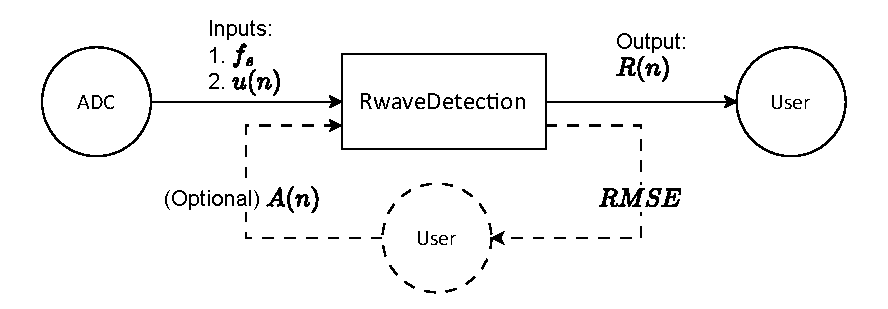
\includegraphics[width=0.8\textwidth]{SystemContextFigure}
\caption{System Context}
\label{Fig_SystemContext} 
\end{center}
\end{figure}

\begin{itemize}
\item User Responsibilities:
\begin{itemize}
\item Provide integer ADC sample frequency $f_s$
\item Provide discrete time domain ECG signal real sequence $u$ sampled from ADC
\item (Optional) Provide correctly annotated data real sequence $A$
\end{itemize}
\item \progname{} Responsibilities:
\begin{itemize}
\item Detect data type mismatch, such as a string of characters instead of a
  real number
\item Return the integer sequence index of each R-wave peak $R$ detected from
$u$
\item Render a graph that shows $u$ and $R$ at the same time
\item Return the $\text{RMSE}$ between $A$ and $R$ if required
\end{itemize}
\end{itemize}

\subsection{User Characteristics} \label{SecUserCharacteristics}

The end user of RwaveDetection needs to have a basic understanding of the QRS
complex in ECG.  Advanced user who hopes to evaluate the accuracy of the system
should have an understanding of undergraduate level mathematics.

\subsection{System Constraints}

RwaveDetection should be able to process data in real time and it can be used in
various low performance embedded devices, so it requires a Low-Level programming
language to ensure efficiency and compatibility.

\section{Specific System Description}

This section first presents the problem description, which gives a high-level
view of the problem to be solved.  This is followed by the solution
characteristics specification, which presents the assumptions, theories,
definitions and finally the instance models.

\subsection{Problem Description} \label{Sec_pd}

\progname{} is intended to find the R-wave peak position accurately from single
channel ECG data containing clutter and noise.

\subsubsection{Terminology and  Definitions}

This subsection provides a list of terms that are used in the subsequent
sections and their meaning, with the purpose of reducing ambiguity and making it
easier to correctly understand the requirements:

\begin{itemize}

\item QRS complex: the combination of three of the graphical deflections seen on
a typical electrocardiogram (ECG or EKG)\cite{wiki:QRS_complex}
\item R-wave: represents the peak of ventricular depolarization
\item Filter: a device or process that removes some unwanted components or
features from a signal\cite{wiki:Filter_(signal_processing)}
\item Utility frequency: the nominal frequency of the oscillations of
alternating current (AC) in a wide area synchronous grid transmitted from a
power station to the end-user.\cite{wiki:Utility_frequency}

\end{itemize}

\subsubsection{Physical System Description} \label{sec_phySystDescrip}

The physical system of \progname{}, includes the following elements:

\begin{itemize}

\item[PS1:] The heart generates electrical impulses that propagate through the
body, causing voltage differences at the skin surface.

\item[PS2:] Electrodes placed on the body detect the electrical signals from the
heart.  These signals are captured in the form of voltage differences between
the electrode pairs.

\item[PS3:] Noise elements such as muscle artifacts, motion artifacts, and
electrical interference from external sources (e.g., power lines) can corrupt
the ECG signal.

\end{itemize}

% \begin{figure}[h!] \begin{center} %\rotatebox{-90}
% {
%  \includegraphics[width=0.5\textwidth]{<FigureName>}
% }
% \caption{\label{<Label>} <Caption>} \end{center} \end{figure}

\subsubsection{Goal Statements}

\begin{itemize}

\item[GS\refstepcounter{goalnum}\thegoalnum \label{G_find_index}:] Given a
single-channel unfiltered ECG signal, find the index of each R-wave peak.

\item[GS\refstepcounter{goalnum}\thegoalnum \label{G_calculate_RMSE}:] Given
correct annotated data, calculate the RMSE between each detected R-wave peak
time and annotated time.

\end{itemize}

\subsection{Solution Characteristics Specification}

% \plt{This section specifies the information in the solution domain of the
%   system to be developed. This section is intended to express what is required
%   in such a way that analysts and stakeholders get a clear picture, and the
%   latter will accept it. The purpose of this section is to reduce the problem
%   into one expressed in mathematical terms. Mathematical expertise is used to
%   extract the essentials from the underlying physical description of the
%   problem, and to collect and substantiate all physical data pertinent to the
%   problem.}

% \plt{This section presents the solution characteristics by successively
%   refining models.  It starts with the abstract/general Theoretical Models
%   (TMs) and refines them to the concrete/specific Instance Models (IMs).  If
%   necessary there are intermediate refinements to General Definitions (GDs).
%   All of these refinements can potentially use Assumptions (A) and Data
%   Definitions (DD). TMs are refined to create new models, that are called GMs
%   or IMs. DDs are not refined; they are just used. GDs and IMs are derived, or
%   refined, from other models. DDs are not derived; they are just given. TMs
%   are also just given, but they are refined, not used.  If a potential DD
%   includes a derivation, then that means it is refining other models, which
%   would make it a GD or an IM.}

% \plt{The above makes a distinction between ``refined'' and ``used.'' A model
%   is refined to another model if it is changed by the refinement. When we
%   change a general 3D equation to a 2D equation, we are making a refinement,
%   by applying the assumption that the third dimension does not matter. If we
%   use a definition, like the definition of density, we aren't refining, or
%   changing that definition, we are just using it.}

% \plt{The same information can be a TM in one problem and a DD in another.  It
%   is about how the information is used.  In one problem the definition of
%   acceleration can be a TM, in another it would be a DD.}

% \plt{There is repetition between the information given in the different chunks
%   (TM, GDs etc) with other information in the document.  For instance, the
%   meaning of the symbols, the units etc are repeated.  This is so that the
%   chunks can stand on their own when being read by a reviewer/user.  It also
%   facilitates reuse of the models in a different context.}

% \noindent \plt{The relationships between the parts of the document are show in
%   the following figure.  In this diagram ``may ref'' has the same role as
%   ``uses'' above.  The figure adds ``Likely Changes,'' which are able to
%   reference (use) Assumptions.}

\begin{figure}[H]
  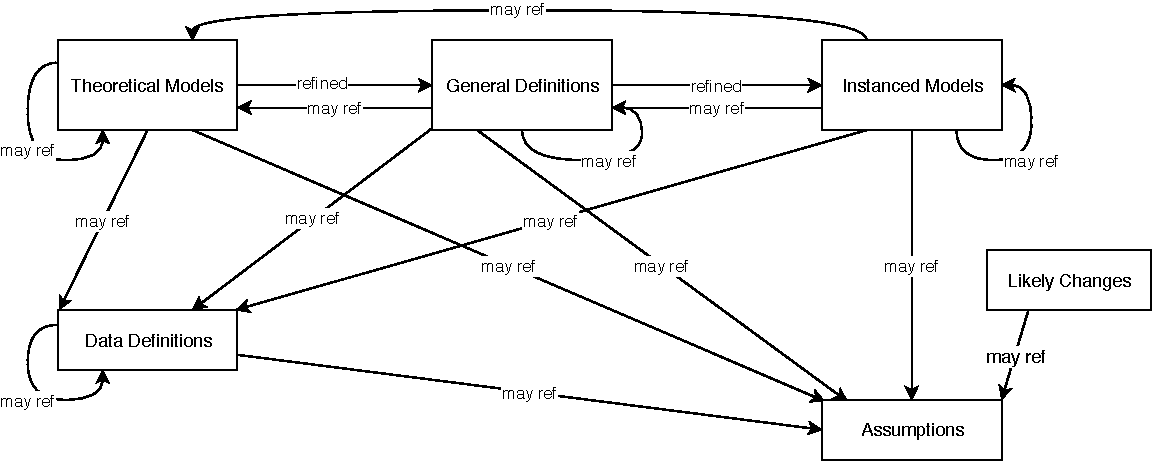
\includegraphics[scale=0.9]{RelationsBetweenTM_GD_IM_DD_A.pdf}
\end{figure}

The instance models that govern \progname{} are presented in
Subsection~\ref{sec_instance}.  The information to understand the meaning of the
instance models and their derivation is also presented, so that the instance
models can be verified.

% \subsubsection{Types}

% \plt{This section is optional. Defining types can make the document easier to
% understand.}

\subsubsection{Assumptions} \label{sec_assumpt}

This section simplifies the original problem and helps in developing the
theoretical model by filling in the missing information for the physical system.
The numbers given in the square brackets refer to the theoretical model [TM],
general definition [GD], data definition [DD], instance model [IM], or likely
change [LC], in which the respective assumption is used.

\begin{itemize}

\item[A\refstepcounter{assumpnum}\theassumpnum \label{A_Nq_frequency}:] The
sampling frequency is not lower than the Nyquist frequency.

\item[A\refstepcounter{assumpnum}\theassumpnum \label{A_filtered_out}:] Noise in
data can be filtered out, within expectations.

\item[A\refstepcounter{assumpnum}\theassumpnum \label{A_naked_eye}:] The R-wave
has peak characteristics that can be discerned by the naked eye.

\item[A\refstepcounter{assumpnum}\theassumpnum \label{A_high_quality}:] The
input ECG signal is of high quality.

\end{itemize}

\newpage

\subsubsection{Theoretical Models}\label{sec_theoretical}

~\newline
\refstepcounter{theorynum}
\noindent
\deftheory
% #2 refname of theory
{TM\thetheorynum}
% #3 label
{Analog Filter Equation}
% #4 equation
{$H(s) = \frac{\sum_{i=0}^{m}{b_is^i}}{\sum_{i=0}^{n}{a_is^i}}$}
% #5 description
{ \leavevmode \\
  $H$ is the transfer function of the filter.  \\
  $s$ is the Laplace variable (complex frequency).  \\
  $b_m$, $b_{m-1}$, $...$, $b_0$ are the numerator coefficients.  \\
  $a_n$, $a_{n-1}$, $...$, $a_0$ are the denominator coefficients, where $a_n
  \neq 0$ to ensure causality and stability.  \\
  $n$ and $m$ represent the highest order of the denominator and numerator
  polynomials, respectively.  Usually, $n \geq m$ to maintain realizability
  (strictly causal system).  }
% #6 Notes
{ Transfer functions are commonly used in the analysis of systems such as
  single-input single-output filters in signal processing, communication theory,
  and control theory.  }
% #7 Source
{
  \url{https://en.wikipedia.org/wiki/Transfer_function}
}
% #8 Referenced by
{
  \tref{Butterworth Filter}
  \tref{Chebyshev Filter}
  \dref{B-trans}
  \dref{FDE}
  \iref{I_find_index}
}
% #9 Preconditions
{ None }
% #1 derivation - not applicable by default
{}

~\newline
\refstepcounter{theorynum}
\noindent
\deftheory
% #2 refname of theory
{TM\thetheorynum}
% #3 label
{Butterworth Filter}
% #4 equation
{$G_n(\omega) = \frac{G_0}{\sqrt{1+(\frac{\omega}{\omega_c})^{2n}}}$}
% #5 description
{ \leavevmode \\
  $G_n$ is the gain function of the $n$th-order Butterworth filter.  \\
  $G_0$ is the DC gain (gain at zero frequency).  \\
  $\omega$ is the angular frequency of the signal.  \\
  $\omega_c$ is the angular cutoff frequency (\si{\hertz}) which defines the
  $-3\si{\decibel}$ point.  \\
  $n$ is the order of the filter.  }
% #6 Notes
{The frequency response of the Butterworth filter is maximally flat (i.e., has
no ripples) in the passband and rolls off towards zero in the stopband.  }
% #7 Source
{
  \url{https://en.wikipedia.org/wiki/Butterworth_filter}
}
% #8 Referenced by
{
  \dref{B-trans}
  \dref{FDE}
  \iref{I_find_index}
}
% #9 Preconditions
{ None }
% #1 derivation - not applicable by default
{}

~\newline
\refstepcounter{theorynum}
\noindent
\deftheory
% #2 refname of theory
{TM\thetheorynum}
% #3 label
{Chebyshev Filter}
% #4 equation
{$G_n(\omega) = \frac{1}{\sqrt{1+\epsilon^2T_n^2(\omega/\omega_c)}}$}
% #5 description
{ \leavevmode \\
$G_n$ is the gain function of the $n$th-order Butterworth filter.  \\
$\epsilon$ is the ripple factor, $|\epsilon| < 1$ \\
$\omega$ is the angular frequency of the signal.  \\
$\omega_c$ is the angular cutoff frequency (\si{\hertz}) which defines the
$-3\si{\decibel}$ point.  \\
$T_n(\frac{\omega}{\omega0})$ is the $n$th order Chebyshev polynomials.  
}
% #6 Notes
{Chebyshev filters have a steeper roll-off than Butterworth filters, and have
either passband ripple (type I) or stopband ripple (type II).  }
% #7 Source
{
  \url{https://en.wikipedia.org/wiki/Chebyshev_filter}
}
% #8 Referenced by
{
  \dref{B-trans}
  \dref{FDE}
  \iref{I_find_index}
}
% #9 Preconditions
{ None }
% #1 derivation - not applicable by default
{}

~\newline
\refstepcounter{theorynum}
\noindent
\deftheory
% #2 refname of theory
{TM\thetheorynum}
% #3 label
{Threshold Detect}
% #4 equation
{ $T[n] = 
\begin{cases}
x[n] & \text{if } x[n] \geq \theta \\
0 & \text{if } x[n] < \theta \end{cases}$ }
% #5 description
{ \leavevmode \\
  $x$ is the input signal.  \\
  $T$ is the output signal.  \\
  $\theta$ is the threshold, which is not guaranteed to be a static number all
  the time and may change as the state changes.  \\
}
% #6 Notes
{threshold comparison detection is a simple signal processing technique where
the input signal is compared to a threshold value.}
% #7 Source
{}
% #8 Referenced by
{
  \iref{I_find_index}
  \iref{I_RMSE}
}
% #9 Preconditions
{ None }
% #1 derivation - not applicable by default
{}

\subsubsection{General Definitions}\label{sec_gendef}

This section collects the laws and equations that will be used in building the
instance models.

~\newline

\noindent
\begin{minipage}{\textwidth}
\renewcommand*{\arraystretch}{1.5}
\begin{tabular}{| p{\colAwidth} | p{\colBwidth}|}
\hline
\rowcolor[gray]{0.9}
Number& GD\refstepcounter{defnum}\thedefnum \label{B-trans}\\
\hline
Label &\bf Bilinear transform \\
\hline
% Units&$MLt^{-3}T^0$\\
% \hline SI Units&\si{\watt\per\square\metre}\\
% \hline
Equation&$s \approx \frac{2}{T_s} \cdot \frac{z-1}{z+1}$  \\
\hline
Description & The bilinear transform is used in digital signal processing and
discrete-time control theory to transform continuous-time system representations
to discrete-time.  \\
& $s$ is the Laplace variable (complex frequency).  \\
& $z$ is the complex frequency variable in the Z-domain.  \\
& $T_s$ is the sampling period.  \\
& When \aref{A_Nq_frequency} is satisfied, this equation represents replacing
all $s$ terms in $H(s)$ S-domain transfer function directly with $\frac{2}{T}
\cdot \frac{z-1}{z+1}$, after doing this we can get Z-domain transfer function
H(z).  \\
& Analog filters in \tref{Butterworth Filter} and \tref{Chebyshev Filter} can be
transformed into digital filter in this way. \\
\hline
  Source & \url{https://en.wikipedia.org/wiki/Bilinear_transform} \\
  \hline
  Ref.\ By & \tref{Analog Filter Equation}, \tref{Butterworth Filter},
  \tref{Chebyshev Filter}, \dref{FDE}, \dref{Differential filter},
  \iref{I_find_index}\\
  \hline
\end{tabular}
\end{minipage}\\

~\newline

\noindent
\begin{minipage}{\textwidth}
\renewcommand*{\arraystretch}{1.5}
\begin{tabular}{| p{\colAwidth} | p{\colBwidth}|}
\hline
\rowcolor[gray]{0.9}
Number& GD\refstepcounter{defnum}\thedefnum \label{FDE}\\
\hline
Label &\bf Filter Difference Equation \\
\hline
% Units&$MLt^{-3}T^0$\\
% \hline SI Units&\si{\watt\per\square\metre}\\
% \hline
Equation&$H(z)=\frac{\sum_{l=0}^{N}b_lz^{-l}}{1 + \sum_{k=1}^{M}a_kz^{-k}}
\leftrightarrow y[n] = -\sum_{k=1}^{M}a_ky[n-k] + \sum_{l=0}^{N}b_lx[n-l]$  \\
\hline
Description & $x[n]$ is the input signal at the $n$-th time sample.  \\
& $y[n]$ is the output signal at the $n$-th time sample.  \\
& $b_l$ is the coefficients for the input signal.  \\
& $a_k$ is the coefficients for the output signal.  \\
& $N$ is the maximum delay for the input signal.  \\
& $M$ is the maximum delay for the output signal.  \\
& $z$ is the complex frequency variable in the Z-domain.  \\
& This equation reflects the conversion relationship between the difference
equation and the Z-domain transfer function $H(z)$ comes from \dref{B-trans}. \\

\hline
  Source & \url{https://en.wikipedia.org/wiki/Digital_filter} \\
  \hline
  Ref.\ By & \tref{Analog Filter Equation}, \tref{Butterworth Filter},
  \tref{Chebyshev Filter}, \dref{B-trans}, \dref{Differential filter},
  \iref{I_find_index}\\
  \hline
\end{tabular}
\end{minipage}\\

~\newline

\noindent
\begin{minipage}{\textwidth}
\renewcommand*{\arraystretch}{1.5}
\begin{tabular}{| p{\colAwidth} | p{\colBwidth}|}
\hline
\rowcolor[gray]{0.9}
Number& GD\refstepcounter{defnum}\thedefnum \label{Differential filter}\\
\hline
Label &\bf Differential filter \\
\hline
% Units&$MLt^{-3}T^0$\\
% \hline SI Units&\si{\watt\per\square\metre}\\
% \hline
Equation&$y[n]=\frac{1}{8}(2x[n]+x[n-1]-x[n-3]-2x[n-4])$  \\
\hline
Description & $x[n]$ is the input signal at the $n$-th time sample.  \\
& $y[n]$ is the output signal at the $n$-th time sample.  \\
& The five-point differentiation formula is a numerical method used to
approximate the derivative of a discrete signal.  This filter is actually a
special digital filter using difference equations in \dref{FDE}.  \\
& In this program, differential filter can be used to enhance the slope of the
QRS complex.  \\
\hline
  Source & \url{https://en.wikipedia.org/wiki/Digital_filter} \\
  \hline
  Ref.\ By & \tref{Analog Filter Equation}, \iref{I_find_index}\\
  \hline
\end{tabular}
\end{minipage}\\


% \subsubsection*{Detailed derivation of simplified rate of change of
% temperature}

% \plt{This may be necessary when the necessary information does not fit in the
%   description field.} \plt{Derivations are important for justifying a given
%   GD.  You want it to be clear where the equation came from.}

\subsubsection{Data Definitions}\label{sec_datadef}

This section collects and defines all the data needed to build the instance
models. The dimension of each quantity is also given.

~\newline

\noindent
\begin{minipage}{\textwidth}
\renewcommand*{\arraystretch}{1.5}
\begin{tabular}{| p{\colAwidth} | p{\colBwidth}|}
\hline
\rowcolor[gray]{0.9}
Number& DD\refstepcounter{datadefnum}\thedatadefnum \label{d_pos}\\
\hline
Label& \bf Period of sampling\\
\hline
Symbol &$T_s$\\
\hline
% Units& $Mt^{-3}$\\
% \hline
  SI Units & \si{\second}\\
  \hline
  Equation&$T_s = \frac{1}{f_s}$\\
  \hline
  Description & $T_s$ is the period of sampling (\si{\second}).  \\
  & $f_s$ is the frequency of sampling (\si{\hertz}).  \\
  \hline
  Sources&
  \url{https://en.wikipedia.org/wiki/Sampling_(signal_processing)#Sampling_rate}
  \\
  \hline
  Ref.\ By & \dref{B-trans}, \iref{I_find_index}\\
  \hline
\end{tabular}
\end{minipage}\\

% \subsubsection{Data Types}\label{sec_datatypes}

% \plt{This section is optional.  In many scientific computing programs it isn't
%   necessary, since the inputs and outpus are straightforward types, like
%   reals, integers, and sequences of reals and integers.  However, for some
%   problems it is very helpful to capture the type information.}

% \plt{The data types are not derived; they are simply stated and used by other
%   models.}

% \plt{All data types must be used by at least one of the models.}

% \plt{For the mathematical notation for expressing types, the recommendation is
%   to use the notation of~\cite{HoffmanAndStrooper1995}.}

% This section collects and defines all the data types needed to document the
% models. \plt{Modify the examples below for your problem, and add additional
% definitions as appropriate.}

% ~\newline

% \noindent \begin{minipage}{\textwidth} \renewcommand*{\arraystretch}{1.5}
% \begin{tabular}{| p{\colAwidth} | p{\colBwidth}|} \hline \rowcolor[gray]{0.9}
% Type Name & Name for Type\\
%   \hline Type Def & mathematical definition of the type\\
%   \hline Description & description here \\
%   \hline Sources & Citation here, if the type is borrowed from another
%   source\\
%   \hline \end{tabular} \end{minipage}\\

\subsubsection{Instance Models} \label{sec_instance}    

This section transforms the problem defined in Section~\ref{Sec_pd} into one
which is expressed in mathematical terms. It uses concrete symbols defined in
Section~\ref{sec_datadef} to replace the abstract symbols in the models
identified in Sections~\ref{sec_theoretical} and~\ref{sec_gendef}.

The goal \gsref{G_find_index} is solved by \iref{I_find_index} and
\gsref{G_calculate_RMSE} is solved by \iref{I_RMSE}.

~\newline

%Instance Model 1

\noindent
\begin{minipage}{\textwidth}
\renewcommand*{\arraystretch}{1.5}
\begin{tabular}{| p{\colAwidth} | p{\colBwidth}|}
  \hline
  \rowcolor[gray]{0.9}
  Number& IM\refstepcounter{instnum}\theinstnum \label{I_find_index}\\
  \hline
  Label& \bf Algorithm to detect R-wave peak index\\
  \hline
  Input& $u$, $f_s$, $N$ \\
  \hline
  Output&
  \begin{equation}
    u_f[n] = -\sum_{k=1}^{M}a_ku_f[n-k] + \sum_{l=0}^{N}b_lu[n-l] \nonumber
  \end{equation}\\
  &\begin{equation} u_w[n] = \frac{1}{W}\sum_{k=0}^{W-1}u_f[n-k]^2 \nonumber
  \end{equation}\\
  &\begin{equation} u_{th}[n] = 
      \begin{cases}
        u_w[n] & \text{if } u_w[n] \geq \theta \\
        0 & \text{if } u_w[n] < \theta \end{cases} \nonumber \end{equation}\\
  &\begin{equation} R[i] = \arg\max_{n}{u_{th}[n]}\nonumber \end{equation}\\
  \hline
  Description& $u$ is the sequence of original ECG signal input data.  \\
  & $a$ and $b$ are sequence of digital filter parameters.  \\
  & $M$ and $N$ are the length of filter parameters.  \\
  & $W$ is the window size of sliding window integral. This size needs to be
  adjusted manually.  \\
  & $\theta$ is the R-wave detecting threshold, which is designed to be
  automatically adjusted by the program.   \\
  & $R$ is the final output of the program, which is a sequence of R-wave index
  we hope to detect in \gsref{G_find_index}.  \\
  \hline
  Sources& \url{https://en.wikipedia.org/wiki/Pan%E2%80%93Tompkins_algorithm} \\
  \hline
  Ref.\ By & \tref{Analog Filter Equation}, \tref{Butterworth Filter},
  \tref{Chebyshev Filter}, \tref{Threshold Detect}, \dref{B-trans}, \dref{FDE},
  \dref{Differential filter}, \ddref{d_pos}, \iref{I_RMSE}\\
  \hline
\end{tabular}
\end{minipage}\\

\subsubsection*{Details of \iref{I_find_index}}

When calculating $u_f$, The filter parameters $a$ and $b$ are linear
combinations of a series of filter parameters from \dref{B-trans}.  The sequence
of filters including low-pass and high-pass filter from \tref{Butterworth
Filter} and \tref{Chebyshev Filter} and differential filter from
\dref{Differential filter}.  

We use the square function and sliding window integral to calculate $u_w$, in
this way the R-wave can be amplified and the signal can be smoothed.  

\tref{Threshold Detect} is used when calculating $u_{th}$, so we can focus on
extracting the R-wave and ignore the influence of other signals.  

In the last equation, the variable $n$ has a range limitation, we only take a
continuous period of $n$ where $u_{th}[n]$ is non-zero.  

~\newline

%Instance Model 2

\noindent
\begin{minipage}{\textwidth}
\renewcommand*{\arraystretch}{1.5}
\begin{tabular}{| p{\colAwidth} | p{\colBwidth}|}
  \hline
  \rowcolor[gray]{0.9}
  Number& IM\refstepcounter{instnum}\theinstnum \label{I_RMSE}\\
  \hline
  Label& \bf calculate $\text{RMSE}$ between $A$ and $R$ \\
  \hline
  Input& $A$, $R$, $L$\\
  \hline
  Output&
  \begin{equation}
    \text{RMSE} = \sqrt{\sum_{i=1}^{n}\frac{(A[i]-R[i])^2}{n}} \nonumber
  \end{equation} \\
  \hline
  Description& $A$ is the sequence of integers containing annotated index. \\
  & $R$ is the sequence of integers containing calculated index from
  \iref{I_find_index}. \\
  & $L$ is the length of $A$ and $R$.  Normally they are equal since we assumed
  \aref{A_high_quality}.  \\
  \hline
  Sources& None \\
  \hline
  Ref.\ By & \tref{Threshold Detect}, \iref{I_find_index}\\
  \hline
\end{tabular}
\end{minipage}\\

%~\newline

\subsubsection{Input Data Constraints} \label{sec_DataConstraints}    

Table~\ref{TblInputVar} shows the data constraints on the input output
variables.  The column for physical constraints gives the physical limitations
on the range of values that can be taken by the variable.  The column for
software constraints restricts the range of inputs to reasonable values.  The
software constraints will be helpful in the design stage for picking suitable
algorithms.  The constraints are conservative, to give the user of the model the
flexibility to experiment with unusual situations.  The column of typical values
is intended to provide a feel for a common scenario.  The uncertainty column
provides an estimate of the confidence with which the physical quantities can be
measured.  This information would be part of the input if one were performing an
uncertainty quantification exercise.

The specification parameters in Table~\ref{TblInputVar} are listed in
Table~\ref{TblSpecParams}.

\begin{table}[!h]
  \caption{Input Variables} \label{TblInputVar}
  \renewcommand{\arraystretch}{1.2}
\noindent \begin{longtable*}{l l l l c} 
  \toprule
  \textbf{Var} & \textbf{Physical Constraints} & \textbf{Software Constraints} &
                             \textbf{Typical Value}\\
  \midrule 
  $f_s$ & $f_s > 0$ & $f_{s\text{ min}} \leq f_s \leq f_{s\text{ max}}$ & 360
  \si[per-mode=symbol] {\hertz} \\
  $u$ & $u[n] \geq 0$ & $0 \leq u[n] \leq u_{\text{max}}$ & 0.5\si{\mV} \\
  $N$ & $N > 0$ & $0 < N \leq N_{\text{max}}$ & 36000 \\
  $A$ & $A[n] \geq 0$ & $0 \leq A[n] \leq A_{\text{max}}$ & 15000 \\
  \bottomrule
\end{longtable*}
\end{table}

\begin{table}[!h]
\caption{Specification Parameter Values} \label{TblSpecParams}
\renewcommand{\arraystretch}{1.2}
\noindent \begin{longtable*}{l l} 
  \toprule
  \textbf{Var} & \textbf{Value} \\
  \midrule 
  $f_{s\text{ min}}$ & 100 \si{\hertz}\\
  $f_{s\text{ max}}$ & 5000 \si{\hertz}\\
  $u_{\text{max}}$ & 10 \si{\mV}\\
  $N_{\text{max}}$ & 1,000,000 \\
  $A_{\text{max}}$ & 100,000 \\
  \bottomrule
\end{longtable*}
\end{table}

% \subsubsection{Properties of a Correct Solution} \label{sec_CorrectSolution}

% \noindent A correct solution must exhibit \plt{fill in the details}.
% \plt{These properties are in addition to the stated requirements.  There is no
% need to repeat the requirements here.  These additional properties may not
% exist for every problem.  Examples include conservation laws (like
% conservation of energy or mass) and known constraints on outputs, which are
% usually summarized in tabular form.  A sample table is shown in
% Table~\ref{TblOutputVar}}

% \begin{table}[!h] \caption{Output Variables} \label{TblOutputVar}
% \renewcommand{\arraystretch}{1.2} \noindent \begin{longtable*}{l l} \toprule
% \textbf{Var} & \textbf{Physical Constraints} \\
%   \midrule $T_W$ & $T_\text{init} \leq T_W \leq T_C$ (by~\aref{A_charge}) \\
%   \bottomrule \end{longtable*} \end{table}

% \plt{This section is not for test cases or techniques for verification and
%   validation.  Those topics will be addressed in the Verification and
%   Validation plan.}

\newpage

\section{Requirements}

This section provides the functional requirements, the business tasks that the
software is expected to complete, and the nonfunctional requirements, the
qualities that the software is expected to exhibit.

\subsection{Functional Requirements}

\noindent \begin{itemize}

\item[R\refstepcounter{reqnum}\thereqnum \label{R_basic_filters}:] Implement
basic IIR and FIR filters using difference equations

\item[R\refstepcounter{reqnum}\thereqnum \label{R_Butterworth}:] Implement
parameter derivation of Butterworth filters

\item[R\refstepcounter{reqnum}\thereqnum \label{R_Chebyshev}:] Implement
parameter derivation of Chebyshev filters

\item[R\refstepcounter{reqnum}\thereqnum \label{R_squaring}:] Implement squaring
function

\item[R\refstepcounter{reqnum}\thereqnum \label{R_thresholding}:] Implement
thresholding function

\item[R\refstepcounter{reqnum}\thereqnum \label{R_RMSE}:] Implement RMSE
calculating function

\item[R\refstepcounter{reqnum}\thereqnum \label{R_R_wave_position}:] Combine
mathematical functions and filters to calculate R-wave position

\item[R\refstepcounter{reqnum}\thereqnum \label{R_cal_RMSE}:] Combine annotated
data and detected R-wave index to calculate RMSE

\end{itemize}

\subsection{Nonfunctional Requirements}

\noindent \begin{itemize}

\item[NFR\refstepcounter{nfrnum}\thenfrnum \label{NFR_Usability}:]
  \textbf{Usability} The code uses external automated tools to generate user
  manuals.

\item[NFR\refstepcounter{nfrnum}\thenfrnum \label{NFR_Maintainability}:]
  \textbf{Maintainability} The code is tested with complete verification and
  validation plan.

\item[NFR\refstepcounter{nfrnum}\thenfrnum \label{NFR_Portability}:]
  \textbf{Portability} Write cross-platform and portable code, works on at least
  Linux, Windows.

\item[NFR\refstepcounter{nfrnum}\thenfrnum \label{NFR_Reusability}:]
  \textbf{Reusability} The code is modularized.

\end{itemize}

% \subsection{Rationale}

% \plt{Provide a rationale for the decisions made in the documentation.
% Rationale should be provided for scope decisions, modelling decisions,
% assumptions and typical values.}

\section{Likely Changes}    

\noindent \begin{itemize}

\item[LC\refstepcounter{lcnum}\thelcnum\label{LC_filters}:] The types of digital
filters such as \tref{Butterworth Filter} and \tref{Chebyshev Filter} may be
increased according to actual needs

\item[LC\refstepcounter{lcnum}\thelcnum\label{LC_parameters}:] Some specific
parameters in \iref{I_find_index} may be changed, such as the default filter
order number, cutoff frequency, window size etc.

\item[LC\refstepcounter{lcnum}\thelcnum\label{LC_database}:] Some ECG data other
than MITBIH may be used.

\end{itemize}

\section{Unlikely Changes}    

\noindent \begin{itemize}

\item[LC\refstepcounter{lcnum}\thelcnum\label{LC_convert}:] The method of
converting continuous-time systems to discrete-time systems will be bilinear
transform in \dref{B-trans} and does not change.

\end{itemize}

\section{Traceability Matrices and Graphs}

The purpose of the traceability matrices is to provide easy references on what
has to be additionally modified if a certain component is changed.  Every time a
component is changed, the items in the column of that component that are marked
with an ``X'' may have to be modified as well.  Table~\ref{Table:trace} shows
the dependencies of theoretical models, general definitions, data definitions,
and instance models with each other. Table~\ref{Table:R_trace} shows the
dependencies of instance models, requirements, and data constraints on each
other. Table~\ref{Table:A_trace} shows the dependencies of theoretical models,
general definitions, data definitions, instance models, and likely changes on
the assumptions.

\begin{table}[htbp!]
\centering
\begin{tabular}{|c|c|c|c|c|}
\hline
	& \aref{A_Nq_frequency}& \aref{A_filtered_out}& \aref{A_naked_eye}&
	\aref{A_high_quality} \\
\hline
\tref{Analog Filter Equation} & & X& &  \\ \hline
\tref{Butterworth Filter}     & & X& &  \\ \hline
\tref{Chebyshev Filter}       & & X& &  \\ \hline
\tref{Threshold Detect}       & & X& X&  \\ \hline
\dref{B-trans}                & X& & &  \\ \hline
\dref{FDE}                    & X& & &  \\ \hline
\dref{Differential filter}    & X& & &  \\ \hline
\ddref{d_pos}                 & & & &  \\ \hline
\iref{I_find_index}           & X& X& X& X \\ \hline
\iref{I_RMSE}                 & & X& X& X \\ \hline
\lcref{LC_filters}            & X& & &  \\ \hline
\lcref{LC_parameters}         & X& & X&  \\ \hline
\lcref{LC_database}           & X& X& X& X \\ \hline
\lcref{LC_convert}            & X& & &  \\
\hline
\end{tabular}
\caption{Traceability Matrix Showing the Connections Between Assumptions and Other Items}
\label{Table:A_trace}
\end{table}

\begin{table}[htbp!]
\centering
\begin{tabular}{|c|c|c|c|c|c|c|c|c|c|c|c|c|c|c|c|c|c|c|c|c|c|c|c|}
\hline        
	& \tref{Analog Filter Equation}& \tref{Butterworth Filter}& \tref{Chebyshev
	Filter}& \tref{Threshold Detect}& \dref{B-trans} & \dref{FDE}&
	\dref{Differential filter} & \ddref{d_pos}& \iref{I_find_index}& \iref{I_RMSE}
	\\
\hline
\tref{Analog Filter Equation}  & & & & & X& X& X& & X&  \\ \hline
\tref{Butterworth Filter}      & X& & & & X& X& & & X&  \\ \hline
\tref{Chebyshev Filter}        & X& & & & X& X& & & X&  \\ \hline
\tref{Threshold Detect}        & & & & & & & & & X& X \\ \hline
\dref{B-trans}                 & X& X& X& & & X& & X& X&  \\ \hline
\dref{FDE}                     & X& X& X& & X& & & & X&  \\ \hline
\dref{Differential filter}     & & & & & X& X& & & X&  \\ \hline
\ddref{d_pos}                  & & & & & & & & & X&  \\ \hline
\iref{I_find_index}            & X& X& X& X& X& X& X& X& & X \\ \hline
\iref{I_RMSE}                  & & & & X& & & & & X&  \\
\hline
\end{tabular}
\caption{Traceability Matrix Showing the Connections Between Items of Different Sections}
\label{Table:trace}
\end{table}

\begin{table}[htbp!]
\centering
\begin{tabular}{|c|c|c|}
\hline
	& \iref{I_find_index}& \iref{I_RMSE} \\
\hline
\rref{R_basic_filters}     & X&  \\ \hline
\rref{R_Butterworth}       & X&  \\ \hline
\rref{R_Chebyshev}         & X&  \\ \hline
\rref{R_squaring}          & X&  \\ \hline
\rref{R_thresholding}      & X&  \\ \hline
\rref{R_RMSE}              & & X \\ \hline
\rref{R_R_wave_position}   & X&  \\ \hline
\rref{R_cal_RMSE}          & & X \\
\hline
\end{tabular}
\caption{Traceability Matrix Showing the Connections Between Requirements and Instance Models}
\label{Table:R_trace}
\end{table}

The purpose of the traceability graphs is also to provide easy references on
what has to be additionally modified if a certain component is changed.  The
arrows in the graphs represent dependencies. The component at the tail of an
arrow is depended on by the component at the head of that arrow. Therefore, if a
component is changed, the components that it points to should also be changed.
% Figure~\ref{Fig_ATrace} shows the dependencies of theoretical models, general
% definitions, data definitions, instance models, likely changes, and
% assumptions on each other. Figure~\ref{Fig_RTrace} shows the dependencies of
% instance models, requirements, and data constraints on each other.

% \begin{figure}[h!] \begin{center} %\rotatebox{-90}
%     {
%       \includegraphics[width=\textwidth]{ATrace.png}
%     }
%     \caption{\label{Fig_ATrace} Traceability Matrix Showing the Connections Between Items of Different Sections}
%   \end{center} \end{figure}


% \begin{figure}[h!] \begin{center} %\rotatebox{-90}
%     {
%       \includegraphics[width=0.7\textwidth]{RTrace.png}
%     }
%     \caption{\label{Fig_RTrace} Traceability Matrix Showing the Connections Between Requirements, Instance Models, and Data Constraints}
%   \end{center} \end{figure}

% \section{Development Plan}

% \plt{This section is optional.  It is used to explain the plan for developing
%   the software.  In particular, this section gives a list of the order in
%   which the requirements will be implemented.  In the context of a course this
%   is where you can indicate which requirements will be implemented as part of
%   the course, and which will be ``faked'' as future work.  This section can be
%   organized as a prioritized list of requirements, or it could should the
%   requirements that will be implemented for ``phase 1'', ``phase 2'', etc.}

% \section{Values of Auxiliary Constants}

% \plt{Show the values of the symbolic parameters introduced in the report.}

% \plt{The definition of the requirements will likely call for
% SYMBOLIC\_CONSTANTS.  Their values are defined in this section for easy
% maintenance.}

% \plt{The value of FRACTION, for the Maintainability NFR would be given here.}

\newpage

%\bibliographystyle {plainnat}
\bibliography {../../refs/References, ../../refs/bib}
\bibliographystyle{unsrt}

\end{document}
